\def\year{2017}\relax
%File: formatting-instruction.tex
\documentclass[letterpaper]{article} %DO NOT CHANGE THIS
\usepackage{aaai17}  %Required
\usepackage{times}  %Required
\usepackage{helvet}  %Required
\usepackage{courier}  %Required
\usepackage{url}  %Required
\usepackage{graphicx}  %Required
\usepackage{bm}
\frenchspacing  %Required
\setlength{\pdfpagewidth}{8.5in}  %Required
\setlength{\pdfpageheight}{11in}  %Required
\usepackage{amsmath}
\usepackage{arydshln}
\usepackage{amsfonts}
\usepackage[ruled,vlined]{algorithm2e}
\usepackage{setspace}
\SetKwComment{Comment}{$\triangleright$\ }{}
\usepackage{caption}
\usepackage{subcaption}
\usepackage{float}
\usepackage{setspace}
\usepackage{amsthm}
\usepackage{multirow}
\usepackage{footnote}
\makesavenoteenv{tabular} \makesavenoteenv{table}
\usepackage{caption}
\usepackage{subcaption}
\usepackage{enumitem}
\newtheorem{theorem}{Theorem}
\newtheorem{definition}[section]{Definition}
\newtheorem{proposition}[theorem]{Proposition}
\usepackage{color}
\usepackage{mwe}
%PDF Info Is Required:
  \pdfinfo{
/Title (2017 Formatting Instructions for Authors Using LaTeX)
/Author (AAAI Press Staff)} \setcounter{secnumdepth}{0}
 \begin{document}
% The file aaai.sty is the style file for AAAI Press
% proceedings, working notes, and technical reports.
%
\title{A Reinforcement Learning Framework for Eliciting High Quality Information}
\author{Zehong Hu\textsuperscript{1}, Yang Liu\textsuperscript{2}, Yitao Liang\textsuperscript{3} and Jie Zhang\textsuperscript{1}\\
1 Nanyang Technological University, Singapore\\
2 Harvard University, USA\\
3 University of California, Los Angeles, USA\\}
\maketitle
\begin{abstract}
Peer prediction is a class of mechanisms that help elicit high-quality information from strategic human agents when there is no ground-truth for verifying contributions. Despite its elegant design, peer prediction mechanisms often fail in practice, mostly due to two shortcomings: (1) agents' incentives for exerting effort to produce high-quality information are assumed to be known; (2) agents are modeled as being fully rational. In this paper, we propose the first reinforcement learning (RL) framework in this domain, \emph{Reinforcement Peer Prediction}, to tackle these two limitations. In our framework, we develop a model-free RL algorithm for the data requester to dynamically adjust the incentive level to maximize his revenue, and to pay workers using peer prediction scoring functions. Experiments show significant improvement in data requestor's revenue under different agent models.
\end{abstract}

\section{Introduction}
Crowdsourcing rises as a promising inexpensive method to collect a large amount of training data quickly \cite{snow2008cheap,deng2009imagenet}.
Notwithstanding its high efficiency, one salient concern about crowdsourcing is the quality of the collected information, as it is often too costly to verify workers' contributions.
This problem is called information elicitation without verification~\cite{waggoner2014output}.
A class of incentive mechanisms, collectively called peer prediction, has been developed to solve this problem~\cite{miller2005eliciting,jurca2009mechanisms,witkowski2012robust,witkowski2012peer,radanovic2013robust}.
The core idea of peer prediction is quite simple and elegant -- the mechanism designer financially incentivizes 
workers according to the scoring of their contributions in comparison with their peers'. The payment rules are designed so that each worker reporting truthfully or reporting a high-quality signal is a strict Bayesian Nash Equilibrium for all workers.

Many peer prediction mechanisms adopt the effort-sensitive model to depict agents' trade-off reasoning in contributing high-quality information~\cite{witkowski2013dwelling,dasgupta2013crowdsourced,shnayder2016informed,liu2017sequential}. In these mechanisms, workers are incentivized to exert high efforts to generate high-quality answers.
One critical assumption in those mechanisms is an explicitly-known worker model which includes workers' incentives. Furthermore it is also assumed workers are fully rational, following the utility-maximizing strategy. Unfortunately, neither is true in practice. Firstly, workers' incentives %, or cost,%
to exert high effort can most likely only be known after we, as the mechanism designers, interact with them. Secondly, there is strong evidence showing that human workers are not fully rational~\cite{simon1979rational}, and they are often observed to be deviating from equilibrium strategies in practice \cite{mckelvey1995quantal,jurca2007robust}.

To push peer prediction mechanisms towards being more practical, we propose a reinforcement learning framework, \emph{Reinforcement Peer Prediction}, to interact with workers, so as to (1) incentivize workers to converge to a high effort exertion state, and (2) learn the optimal payment based on workers' contributions at each step.
Nevertheless, we face two main challenges.
Firstly, classic reinforcement learning focuses on the interaction between a single agent and its environment. We, instead, need to effectively consider a multi-agent setting. Immediately a game is formed among workers, because our incentive strategy relies on the comparison between workers' answers and their peers'. Therefore, the evolution of workers' state is a outcome of collective actions from all workers, as well as the environment. Secondly, no ground-truth is available to evaluate either the state of the workers or the rewards in our setting, whereas it is taken as granted in most other reinforcement learning frameworks. Hence, we need to find a proper way to evaluate workers' contributions so that model-free RL algorithms which learn based on the reward signal can be applied.

The main contributions of this paper are as follows.
(1) We propose the first model-free reinforcement peer prediction mechanism.
Our mechanism combines a peer prediction mechanism with reinforcement learning to jointly incentivize workers and learn the optimal incentive level at each step.
(2) Due to the lack of ground-truth, we adopt Bayesian inference to evaluate workers' contributions, and to infer the reward following each action (i.e. offered incentive level). We derive the explicit posterior distribution of workers' contributions and employ Gibbs sampling to eliminate its bias.
(3) In our setting, the inferred contributions are corrupted by noise and only the most recent previous state rather than the current can be observed. We use the online Gaussian process regression to learn the $Q$-function and replace the unknown current state with the pair of the last observed state and incentive level (action).
(4) We conduct empirical evaluation, and the results show that our mechanism is robust, and is able to significantly increase data requester's revenue under different worker models, such as fully rational, bounded rational and learning agent models.

\section{Problem Formulation}
Our proposed mechanism mainly works in the setting where one data requester, at every step, assigns $M$ binary tasks with answer space $\left\{1,2\right\}$ to $N \geq 4$ candidate workers. At step $t$, worker $i$'s labels for the task $j$ is denoted as $L_i^t(j)$, and correspondingly the payment that the data requester pays is denoted as $P^{t}_i(j)$. Note we use $L^{t}_i(j)=0$ to denote task $j$ is not assigned to worker $i$ at step $t$, and naturally under this case $P^{t}_i(j)=0$.
After every step, the data requester collects labels and aggregates them through Bayesian inference~\cite{zheng2017truth}.
Assuming the aggregated labels reach an accuracy of $A_t$,  the revenue for the data requester can then be computed as
\begin{equation}
r_t = F(A_t) - \eta {\sum}_{i=1}^{N}{\sum}_{j=1}^{M}P^t_i(j)
\end{equation}
where $F(\cdot)$ is a non-decreasing monotonic function mapping accuracy to revenue and $\eta$ is a
tunable parameter balancing label quality and costs. Intuitively, the $F(\cdot)$ function needs to be non-deceasing as higher accuracy is preferred and also labels are only useful when their accuracy reaches a certain requirement. Note our framework is robust to any such $F(\cdot)$ function. For instance, it is set as $F(A_t)=A^{10}_t$ in our experiments.
Our goal is to maximize the cumulative revenue $R = \sum_{t=1}^{T} \gamma^{(t-1)} r_t$, where $\gamma\approx 1.0$ is the discount rate and $T$ is the ending time, by making wise choices of actions  (i.e. deciding incentive levels) at each step.

\section{Reinforcement Peer Prediction}
We present \emph{Reinforcement Peer Prediction} in Figure~\ref{ED1}. Note at every step $t$, the payment to worker $i$ for task $j$ is factored as a function over two elements, namely $P^{t}_i(j)=I_t \cdot p^{t}_i(j)$, where $I_t\geq 0$ is the incentive level (scaling factor) learned and computed by our RL algorithm, and
$p^t_i(j)$ is the output of our peer prediction scoring function.
Since the ground-truth is not available, we cannot directly compute the reward (i.e accuracy $A_t$), following each action (i.e. deciding the offered incentive level). 
Thus, we introduce the expected accuracy $\mathbb{E}A_t$ as an unbiased estimator of the real accuracy $A_t$.
It can be calculated as
\begin{equation}
\mathbb{E}A_t = \frac{1}{M}{\sum}_{j=1}^{M} \textrm{Pr}(L^{t}(j) = y^{t}_j)
\end{equation}
where $L^{t}(j)$ and $y^{t}_j$ are the aggregate and true labels at step $t$, respectively. Besides used to aggregate data, Bayesian inference is also used to generate confusion matrices of all workers and the distribution of task labels $\left[\textrm{Pr}(l=1), \textrm{Pr}(l=2)\right]$, with $l$ denoting the ground-truth label.
For worker $i$, his confusion matrix $C_i = [c_{ikg}]_{2\times 2}$ is a measurement of how much efforts he exerts, where $c_{ikg}$ denotes the probability that worker $i$ labels a task in class $k$ as class $g$. Since the accuracy of labels is determined by the overall efforts of workers, we denote the state of the whole worker crowd $s_t$ by workers' average probability of being correct, namely
\begin{equation}
s_t =\frac{1}{N}\cdot {\sum}_{k=1}^2\textrm{Pr}(l=k)\cdot  {\sum}_{i=1}^{N}c_{ikk}.
\end{equation}
After receiving the payment, workers may potentially adjust their strategies in exerting efforts (based on their rationality model), which will lead to the change of their state $s_t$.
However, when deciding the next-step incentive level $I_{t+1}$, we can only estimate the last step state $s_t$.
In other words, the state observation in our mechanism is not only imperfect, but also has one-step delay. This also makes our reinforcement learning problem different from traditional ones.
\begin{figure}[!htb]
        \includegraphics[width=0.45\textwidth]{image/Mechanism}
        %\vspace{2mm}
        \caption{\label{ED1} Illustration of our mechanism}
\end{figure}

\noindent \textbf{Peer Prediction Mechanism:} We adopt the multi-task mechanism proposed by Dasgupta and Ghosh \shortcite{dasgupta2013crowdsourced}.  For each worker-task pair $(i, j)$, it selects a reference worker $k$. Suppose workers $i$ and $k$ have been assigned $d$ other distinct tasks $\{i_1,\ldots,i_d\}$ and $\{k_1,\ldots, k_d\}$, respectively. Then, the payment for worker $i$'s label $L^t_i(j)$ should be
\begin{equation}
p^t_{i}(j)= 1[L^{t}_i(j)=L^{t}_k(j)]- \xi_{i}^d\cdot \xi_{k}^d -\bar{\xi}_{i}^d\cdot \bar{\xi}_{k}^d
\end{equation}
where $\xi_{i}^{d}=\sum_{g=1}^{d}1(L^{t}_k(i_g)=1)/d$ and $\bar{\xi}_{i}^{d}=1-\xi_{i}^{d}$.

\begin{figure*}[htb]
    \centering
    %\hspace{-1mm}
    \begin{subfigure}[t]{0.3\textwidth}
        \centering
        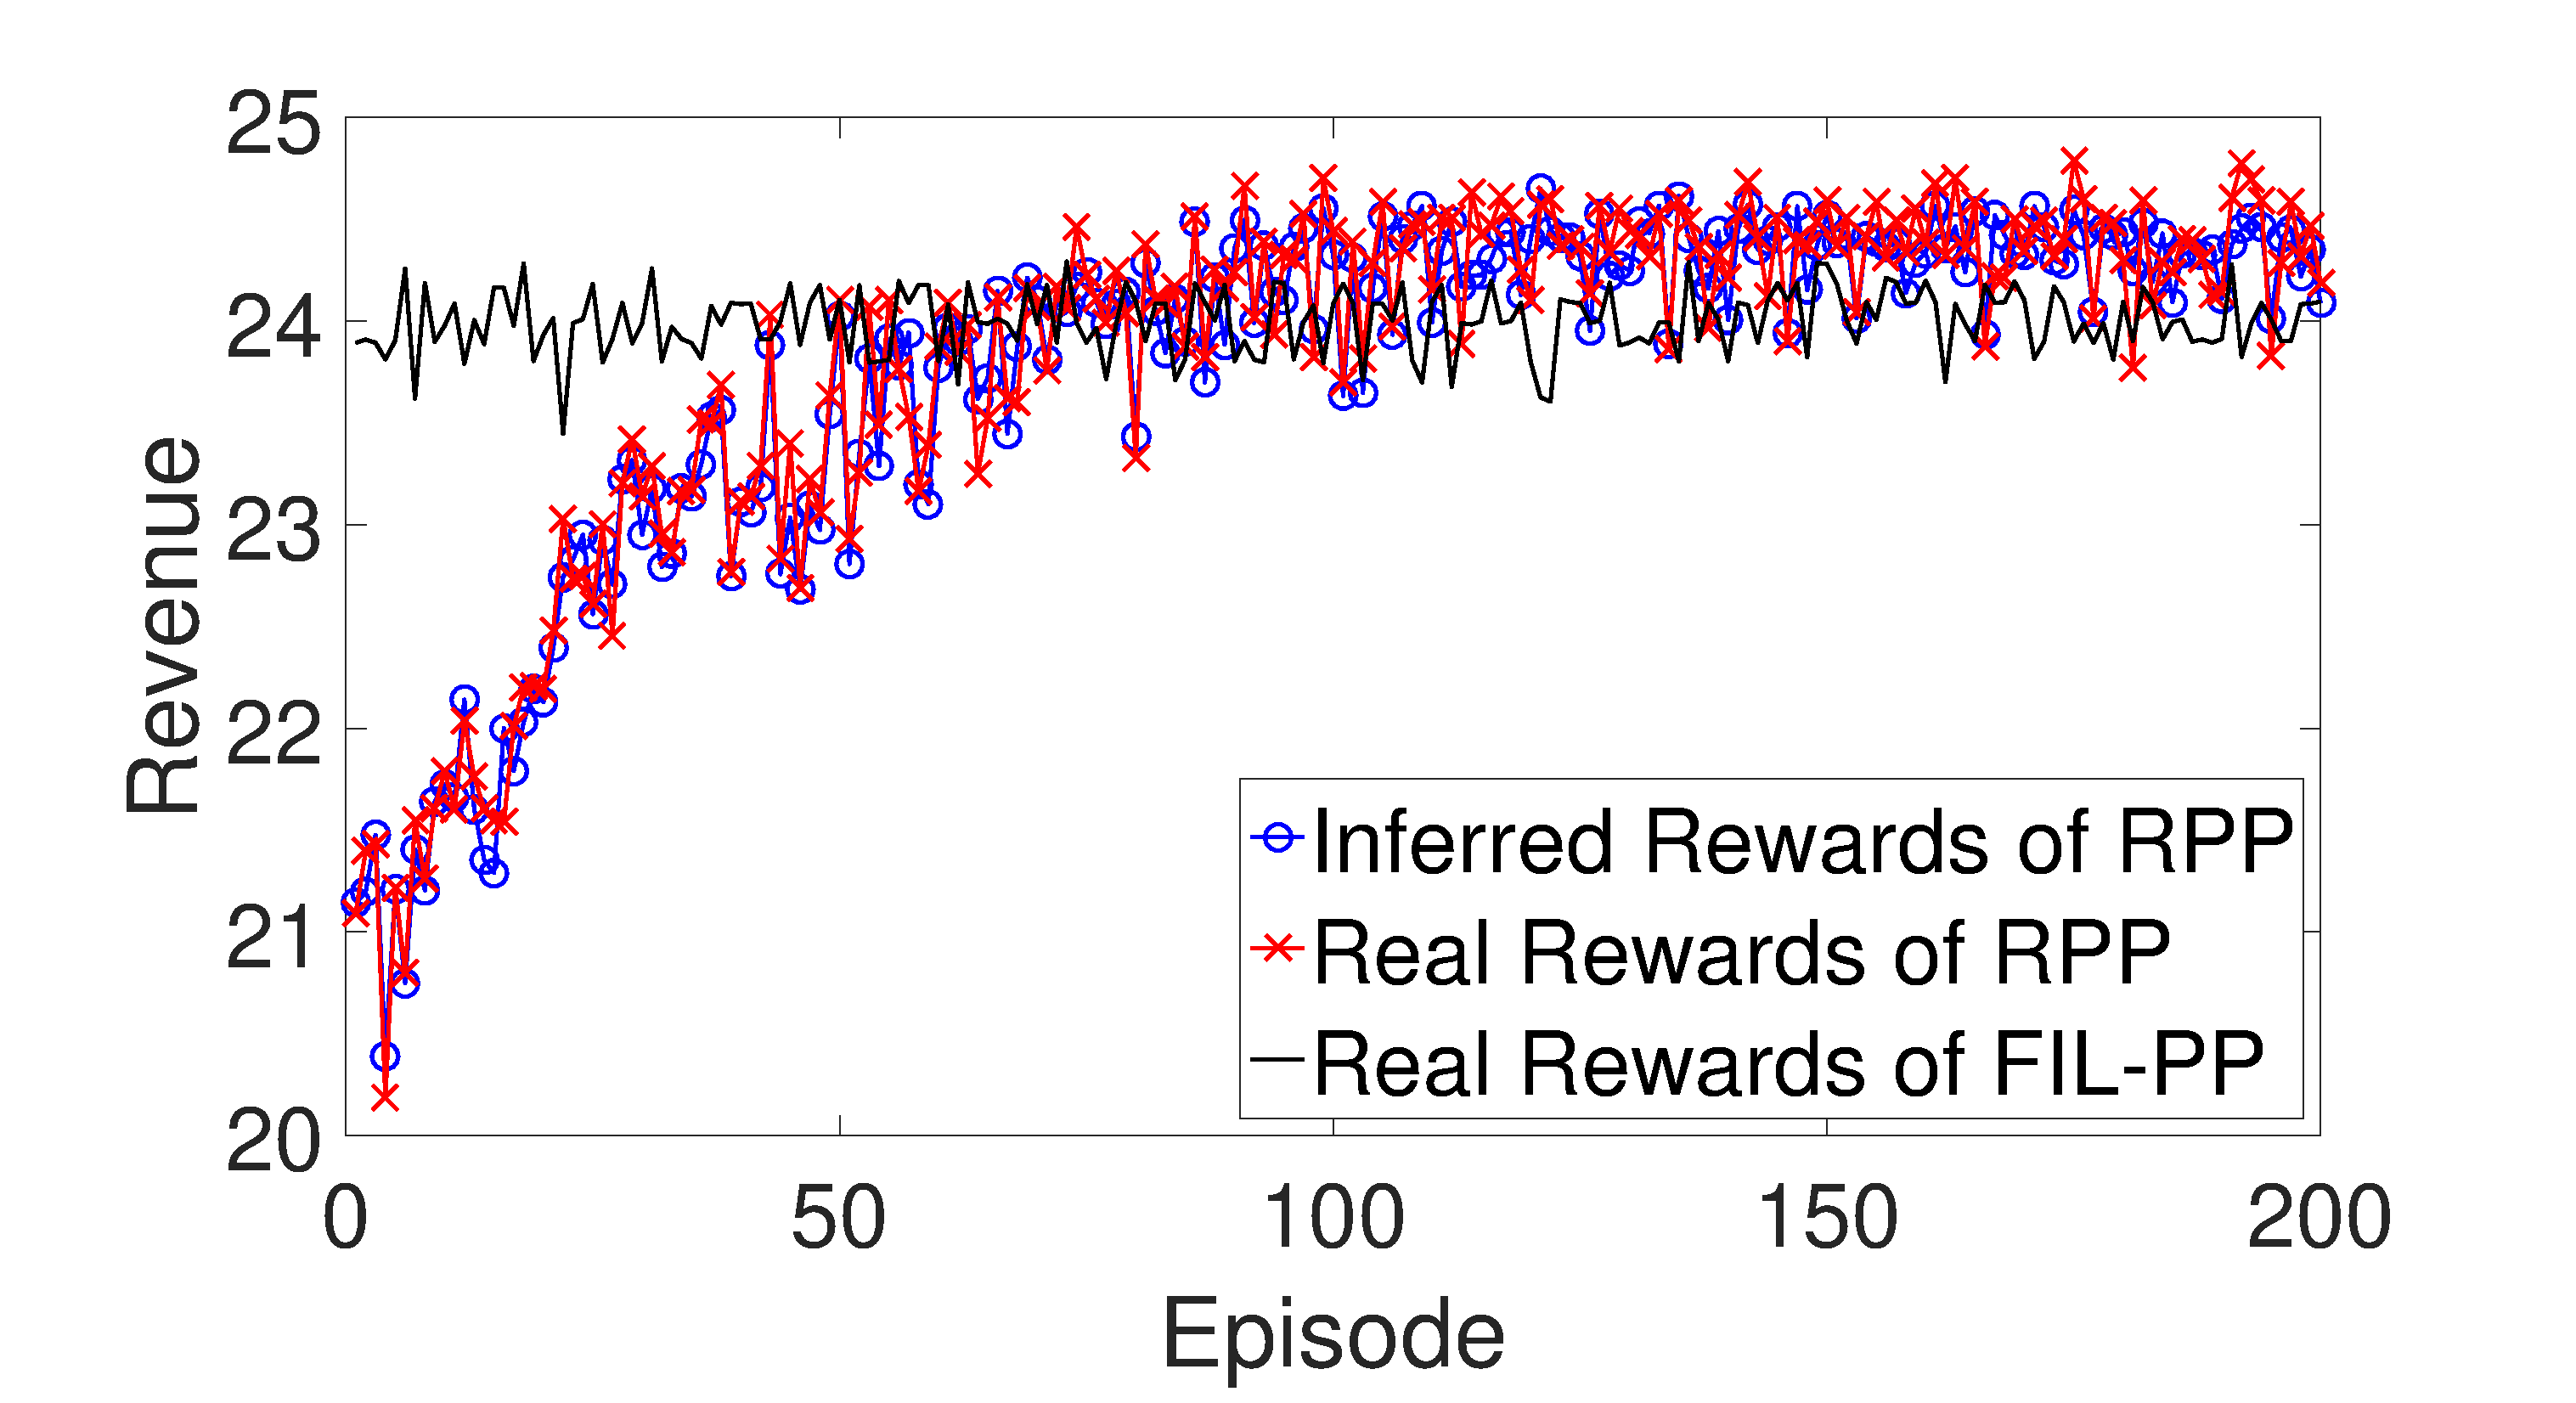
\includegraphics[width=\textwidth]{image/1}
        \caption{\label{E1} Fully Rational Workers}
    \end{subfigure}%
    ~%\hspace{-6mm}
    \begin{subfigure}[t]{0.3\textwidth}
        \centering
        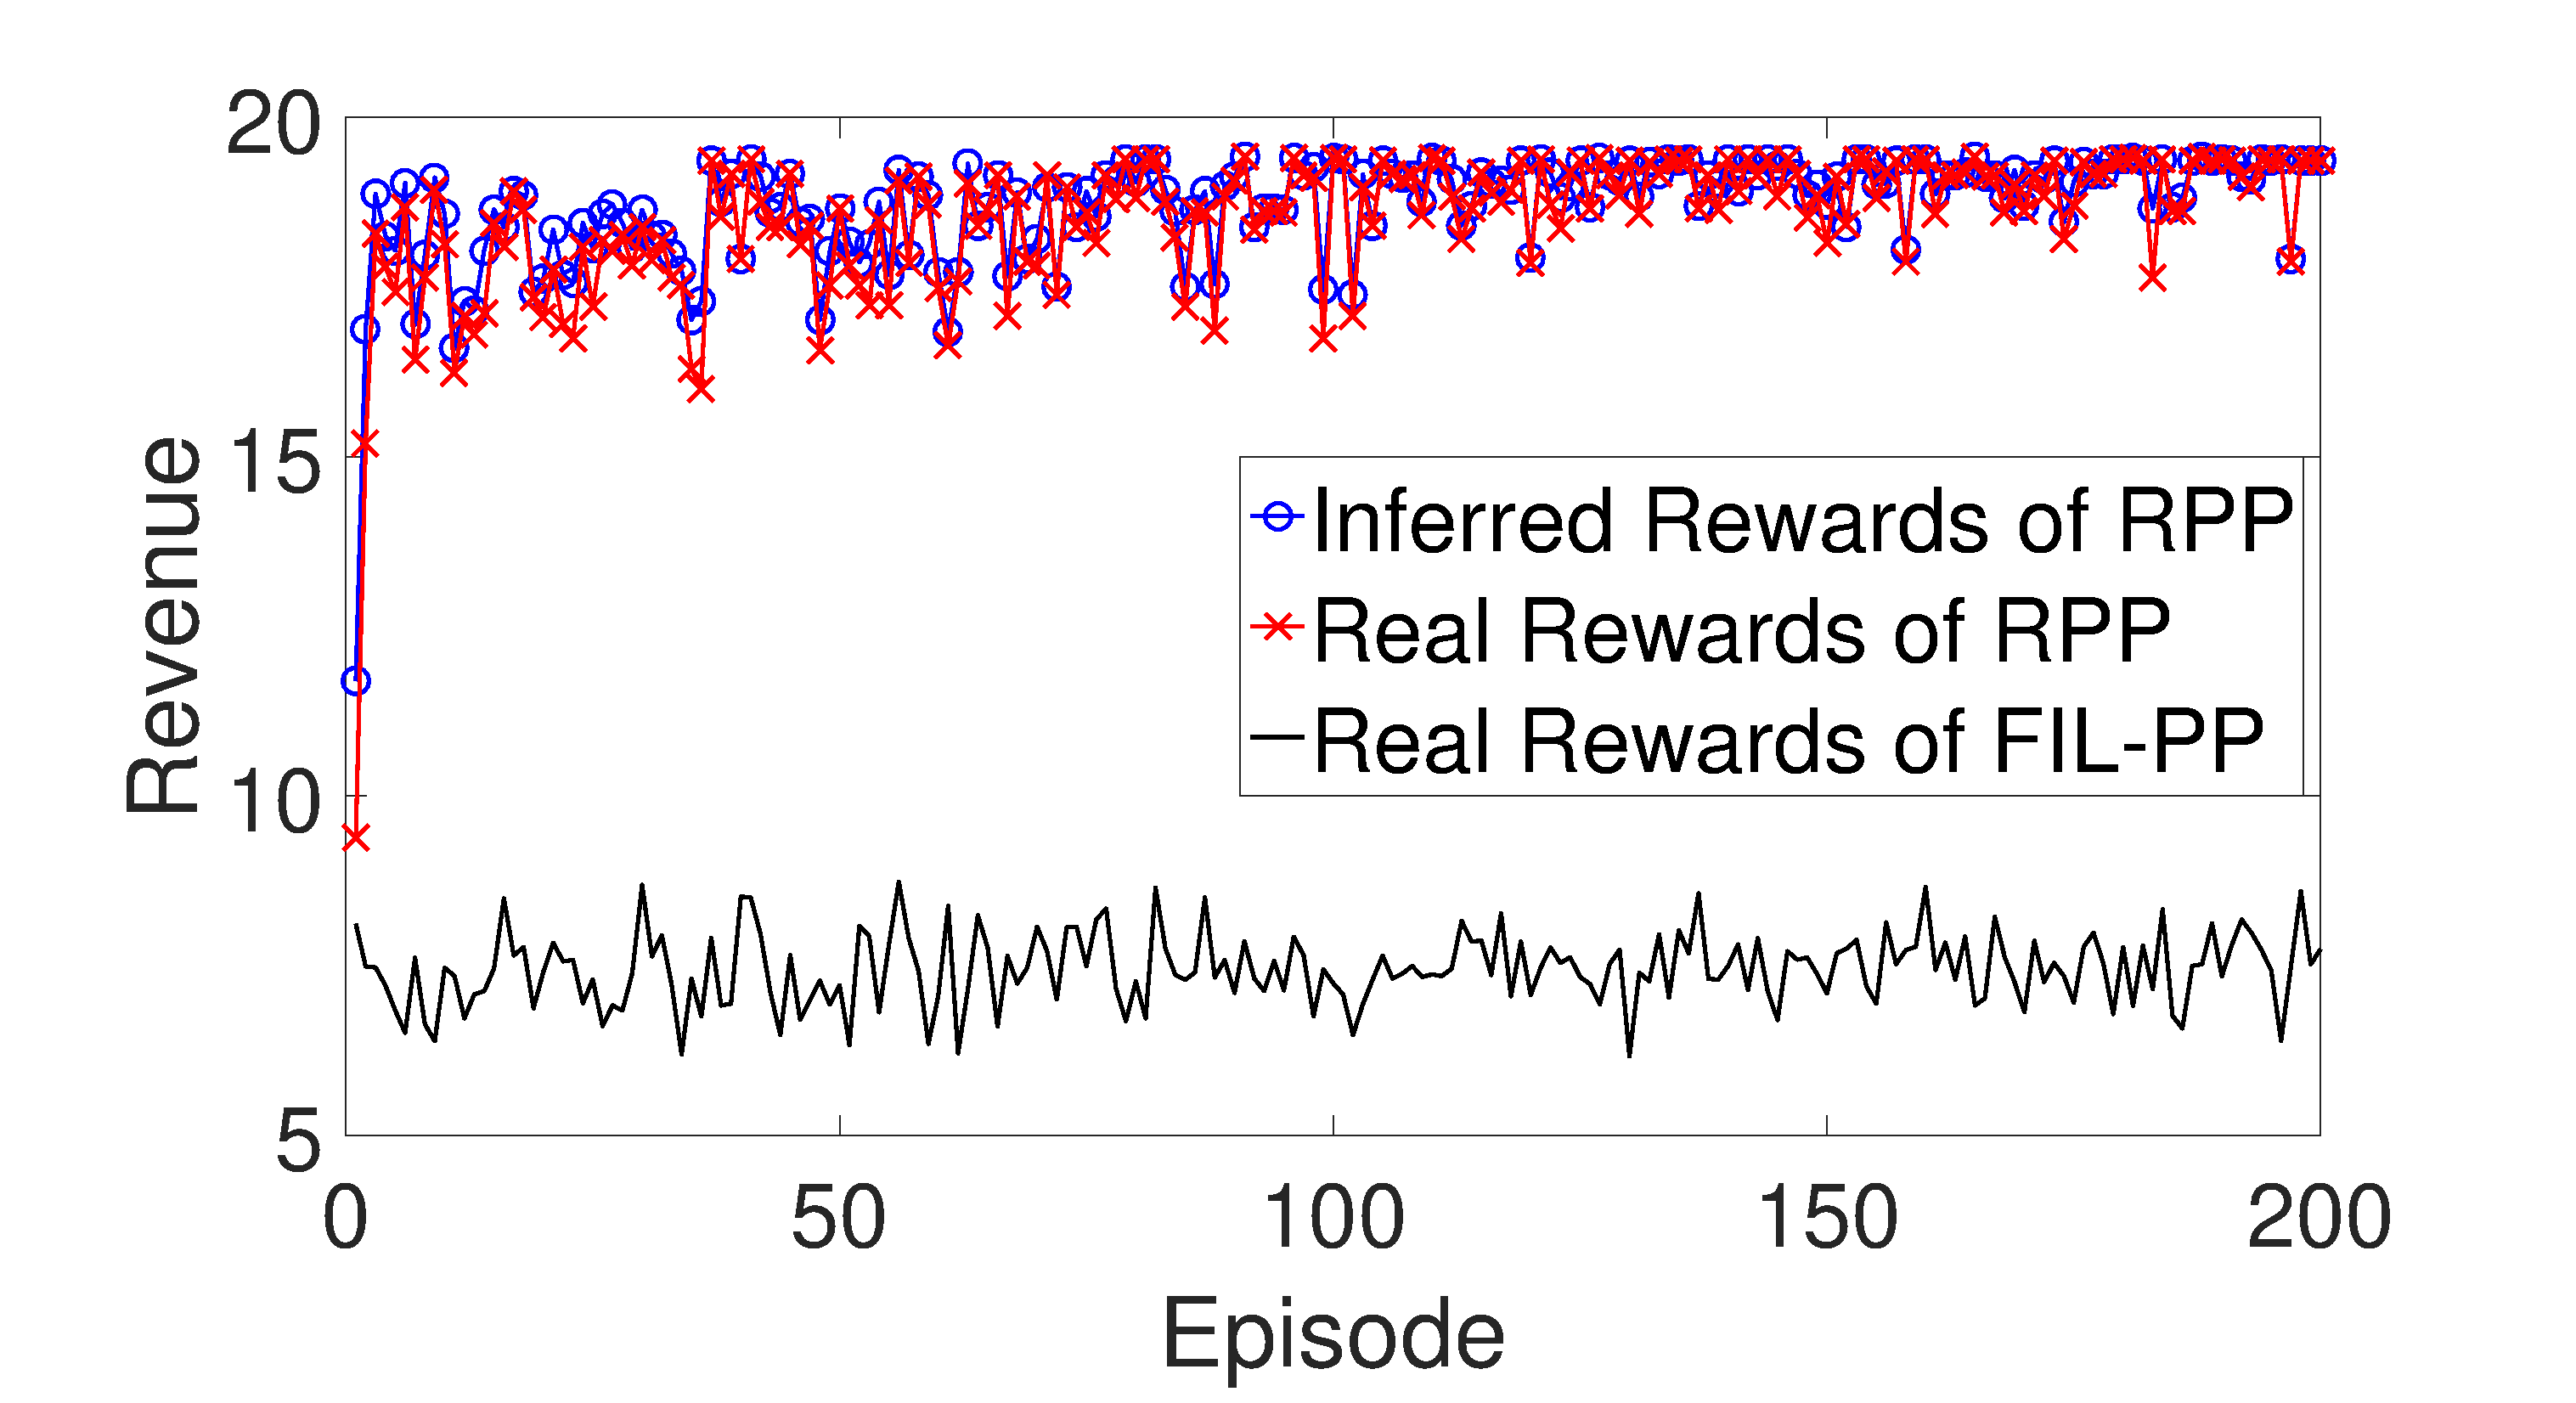
\includegraphics[width=\textwidth]{image/2}
        \caption{\label{E2}  Quantal Response Workers}
    \end{subfigure}
    ~%\hspace{-6mm}
    \begin{subfigure}[t]{0.3\textwidth}
        \centering
        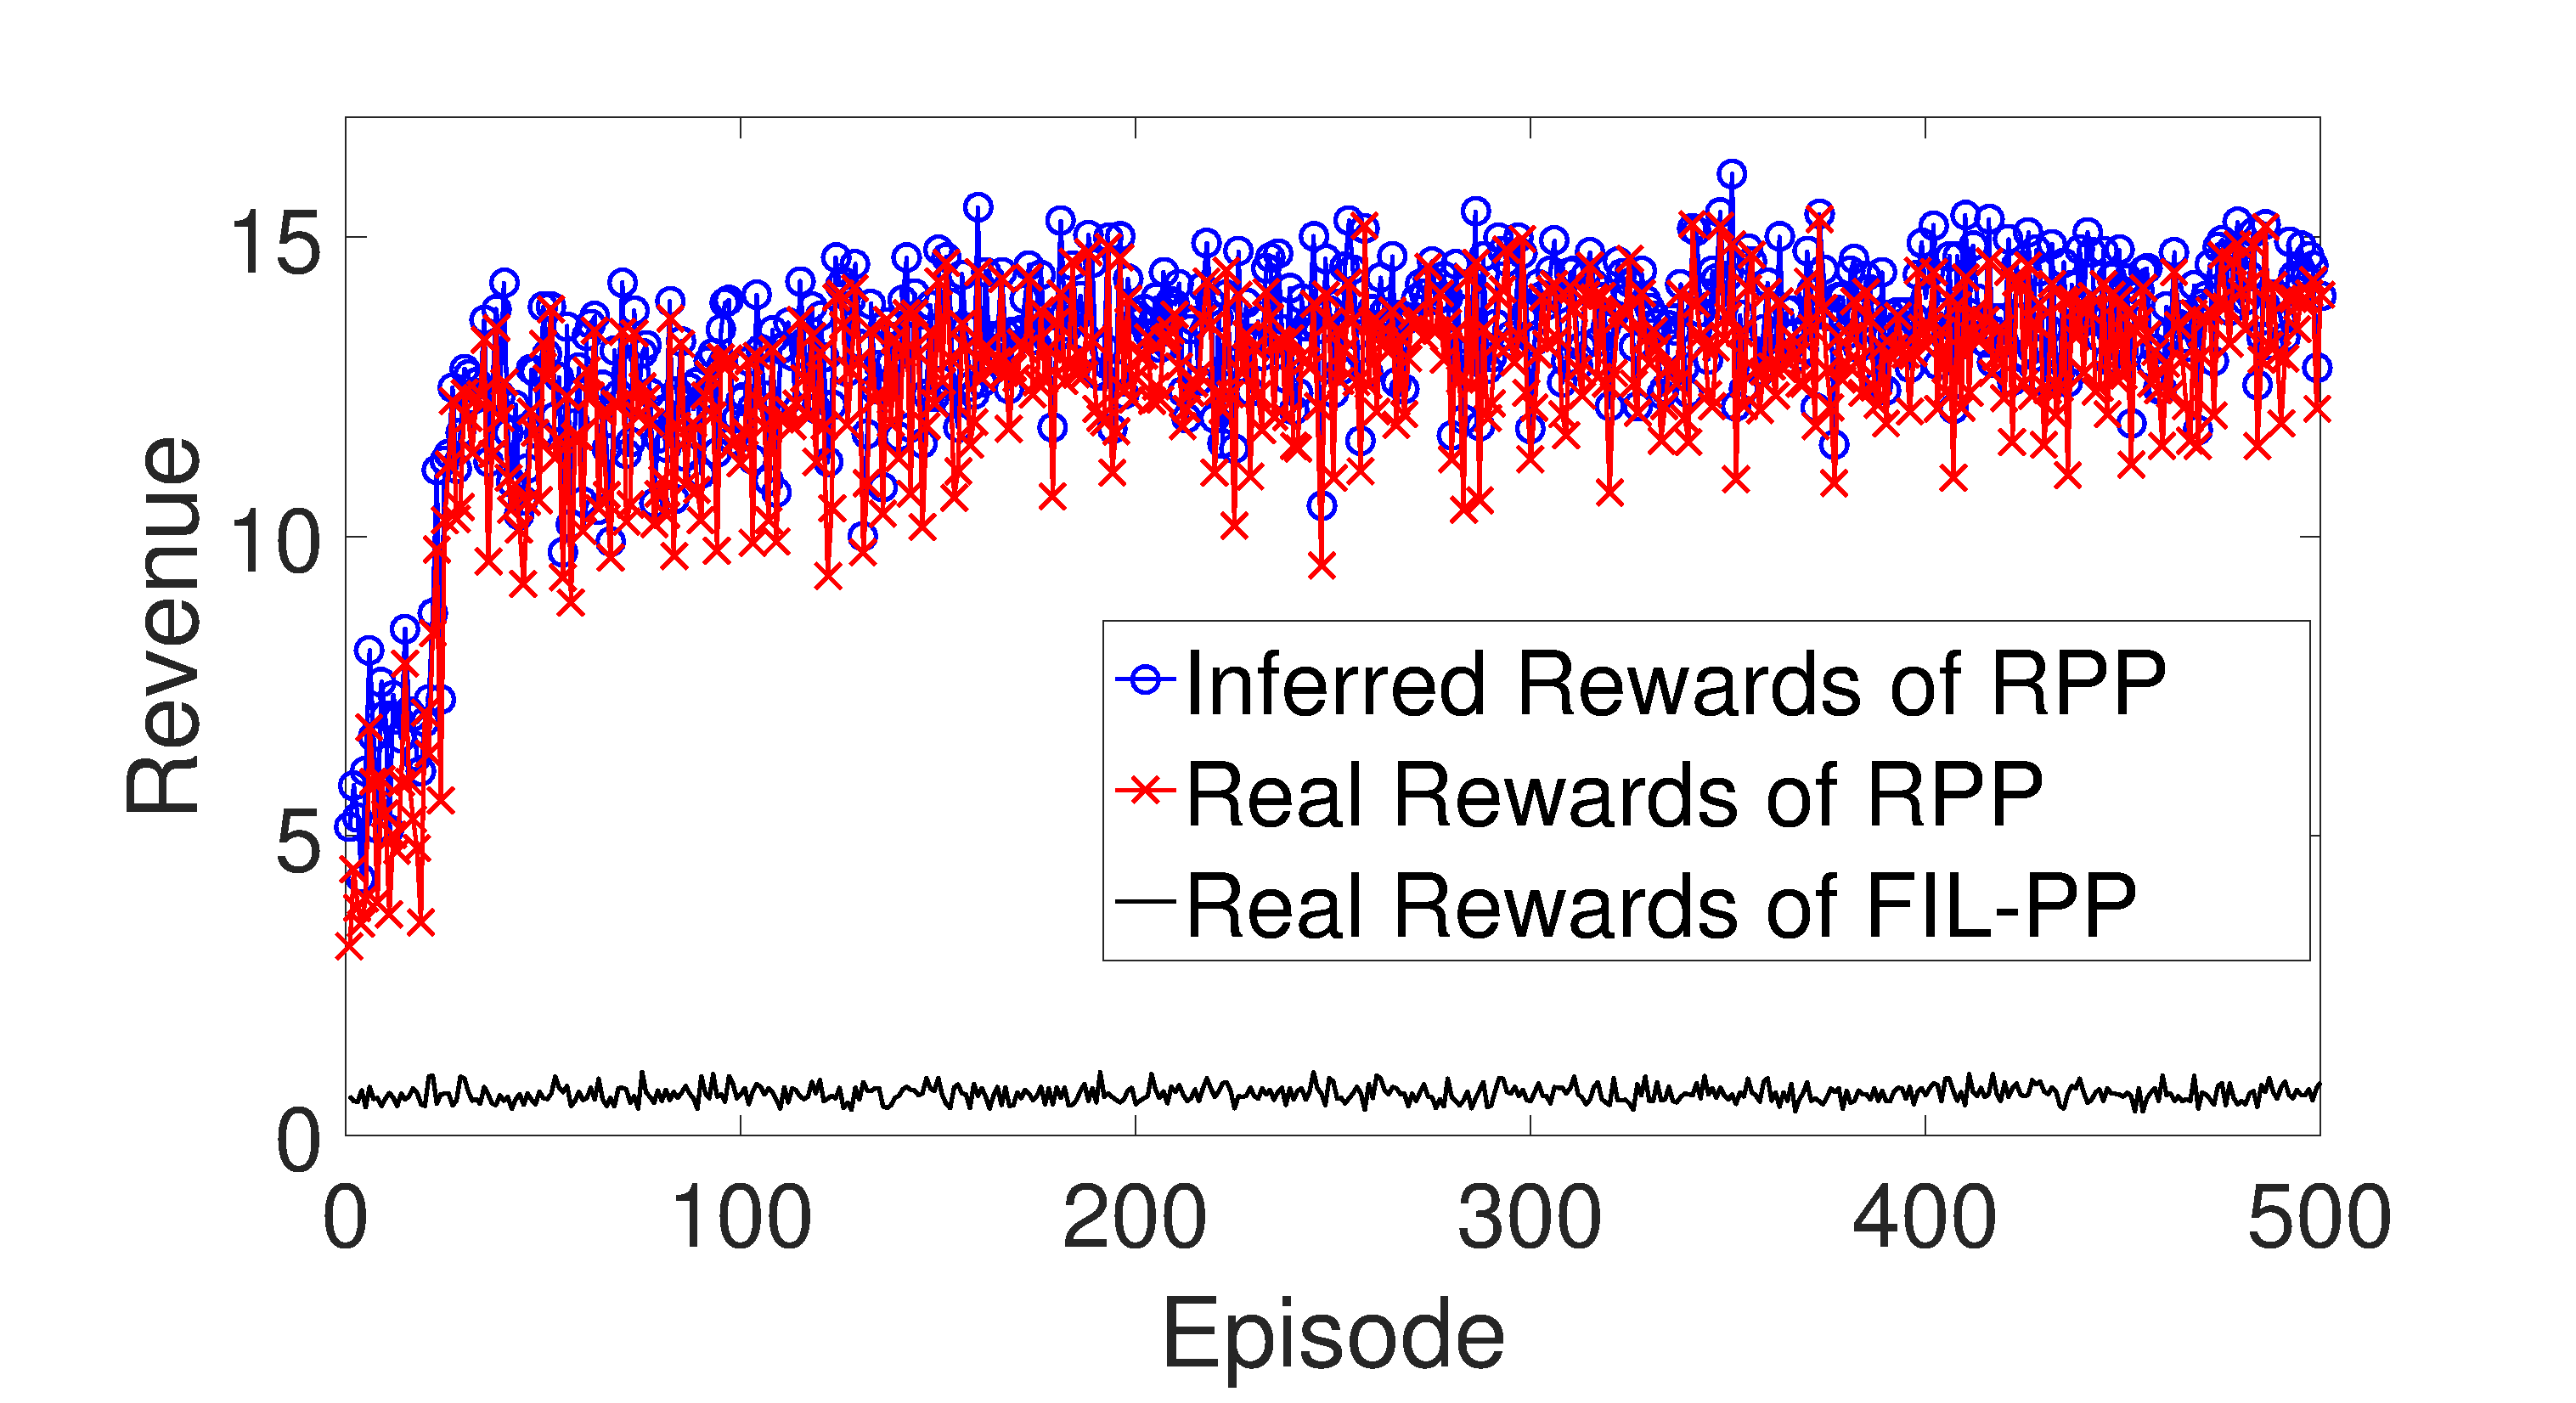
\includegraphics[width=\textwidth]{image/3}
        \caption{\label{E3}  MWUA Workers}
    \end{subfigure}    
    \caption{\label{ED}Experiments on three different worker models}
\end{figure*}

\noindent \textbf{Bayesian Inference:} Suppose the prior distributions are as follows: $c_{ik1}\sim \textrm{Beta}(\alpha^{p}_{ik1},\alpha^{p}_{ik2})$ and $\textrm{Pr}(l=1)\sim \textrm{Beta}(\beta^{p}_{1},\beta^{p}_{2})$. Then, we can explicitly derive the posterior distribution of true labels of assigned tasks, using collected labels from workers, as follows:
\begin{equation}
\label{PostDist}
\begin{split}
&\qquad P(\bm{y}^{t}|\bm{L}^{t})\propto B(\bm{\beta}^{t}){\prod}_{i=1}^{N}{\prod}_{k=1}^{K} B(\bm{\alpha}^{t}_{ik}) \\ 
&\alpha^{t}_{ikg}={\sum}_{j=1}^{M}\delta^{t}_{ijg}\xi^{t}_{jk}+\alpha^{p}_{ikg}, \beta^{t}_k={\sum}_{j=1}^{M}\xi^{t}_{jk}+\beta^{p}_{k}
\end{split}
\end{equation}
where $B(\cdot)$ denotes the beta function, $\delta^{t}_{ijg}=1(L^t_i(j)=g)$ and $\xi^{t}_{jk}= 1(y^{t}_j=k)$. According to Gibbs sampling, we can generate posterior samples via iteratively sampling the conditional probability distribution $P(y^{t}_j=k|\bm{L}, \bm{y}^t_{s\neq j})\propto P(\bm{y}^{t}|\bm{L}^{t})$.
After generating $W$ posterior samples $\bm{y}^{t(1)},\ldots,\bm{y}^{t(W)}$, we can calculate the posterior distribution for the true label of task $j$ as
\begin{equation}
\textrm{Pr}(y^{t}_j=k)=\frac{1}{W}{\sum}_{s=1}^{W}1(y^{t(s)}_j=k).
\end{equation}
Meanwhile, we can decide the aggregated label of task $j$ as
\begin{equation}
L^{t}(j)={\arg\max}_{k\in\{1,2\}}\textrm{Pr}(y^{t}_j=k).
\end{equation}
We can also estimate worker $i$'s confusion matrix as
\begin{equation}
c^{t}_{ikg}=\frac{\alpha_{ikg}^{p}+\sum_{s=1}^{W}\sum_{j=1}^{M}1(y^{t(s)}_j=k)\cdot \delta^{t}_{ijg}}{\sum_{q=1}^2\alpha_{ikq}^{p}+\sum_{s=1}^{W}\sum_{j=1}^{M}1(y^{t(s)}_j=k)}.
\end{equation}


\noindent \textbf{Reinforcement Learning:} Recall that when computing the incentive level $I_{t}$ for step $t$, we do not observe workers' labels and thus cannot estimate the current state $s_{t}$ via Bayesian inference.
Because of it, we resort to the previous state and incentive level to define our  policy $\pi(I_{t}|x_t)$, where $x_t=\langle s_{t-1}, I_{t-1}, t \rangle$.
Then, the $Q$-function of our policy can be calculated as
$Q(x_t, I_t)= \sum_{i=0}^{T-t} \gamma^{i} r_{t+i}$.  %and $Q(x_{T+1}, I_{T+1})=0$.
Since both the state $s_t$ and reward $r_t$ can not be accurately observed, we have to approximate the temporal difference (TD) by assuming that the residual follows a Gaussian process: 
\begin{equation}
Q(x_t, I_t) - \gamma Q(x_{t+1}, I_{t+1}) = r_t + N(x_t,x_{t+1})
\end{equation}
where $N(\cdot)$ is the residual. Then, the Q-function can be learned effectively using the online Gaussian process regression algorithm~\cite{engel2005reinforcement}. Furthermore, we use the classic $\epsilon$-greedy policy to make decisions at every step.


\section{Experiments}
Figure~\ref{ED} 
shows our experimental results on three popular worker models.
Suppose there are four incentive levels, namely $I_t\in \{0.1, 1.0, 5.0, 10.0\}$.
In practice, traditional one-shot peer prediction mechanisms are often implemented with a fixed incentive level.
Here, we set the incentive level as $1.0$ and denote this mechanism with a fixed incentive level as FIL-PP.
By contrast, our reinforcement peer prediction (RPP) mechanism can dynamically learn and adjust the incentive level to maximize data requester's revenue.
Note, in our experiments, rational workers exert  high efforts and report the true labels with probability $0.9$ for any incentive level.
Quantal response workers decide their strategy using the quantal response model, a classic bounded rationality model~\cite{mckelvey1995quantal}.
MWUA workers adapt their strategies via the MWUA model, a classic learning agent model~\cite{chastain2014algorithms}.
Based on all experiment results, we find that our mechanism is robust, and is able to significantly increase data requester's revenue, especially when workers are not fully rational.

\bibliographystyle{named}
\bibliography{ref}
\end{document}
